\documentclass[12pt]{beamer}
\usepackage{../Estilos/BeamerMAF}
\usepackage{arydshln}
%Sección para el tema de beamer, con el theme, usercolortheme y sección de footers
\usetheme{Frankfurt}
\usecolortheme{beaver}
%\useoutertheme{default}
\setbeamercovered{invisible}
% or whatever (possibly just delete it)
\setbeamertemplate{section in toc}[sections numbered]
\setbeamertemplate{subsection in toc}[subsections numbered]
\setbeamertemplate{subsection in toc}{\leavevmode\leftskip=3.2em\rlap{\hskip-2em\inserttocsectionnumber.\inserttocsubsectionnumber}\inserttocsubsection\par}
% \setbeamercolor{section in toc}{fg=blue}
% \setbeamercolor{subsection in toc}{fg=blue}
% \setbeamercolor{frametitle}{fg=blue}
\setbeamertemplate{caption}[numbered]

\setbeamertemplate{footline}
\beamertemplatenavigationsymbolsempty
\setbeamertemplate{headline}{}


\makeatletter
% \setbeamercolor{section in foot}{bg=gray!30, fg=black!90!orange}
% \setbeamercolor{subsection in foot}{bg=blue!30!yellow, fg=red}
% \setbeamercolor{date in foot}{bg=black, fg=white}
\setbeamertemplate{footline}
{
  \leavevmode%
  \hbox{%
  \begin{beamercolorbox}[wd=.333333\paperwidth,ht=2.25ex,dp=1ex,center]{section in foot}%
    \usebeamerfont{section in foot} \insertsection
  \end{beamercolorbox}%
  \begin{beamercolorbox}[wd=.333333\paperwidth,ht=2.25ex,dp=1ex,center]{subsection in foot}%
    \usebeamerfont{subsection in foot}  \insertsubsection
  \end{beamercolorbox}%
  \begin{beamercolorbox}[wd=.333333\paperwidth,ht=2.25ex,dp=1ex,right]{date in head/foot}%
    \usebeamerfont{date in head/foot} \insertshortdate{} \hspace*{2em}
    \insertframenumber{} / \inserttotalframenumber \hspace*{2ex} 
  \end{beamercolorbox}}%
  \vskip0pt%
}







\title{Expansión del potencial de Coulomb}
\subtitle{Tema 4}

\author{M. en C. Gustavo Contreras Mayén}
\date{1 de diciembre de 2021}

\begin{document}
\maketitle
\fontsize{14}{14}\selectfont
\spanishdecimal{.}

\section*{Contenido}
\frame[allowframebreaks]{\tableofcontents[currentsection, hideallsubsections]}


\section{El potencial eléctrico}
\frame{\tableofcontents[currentsection, hideothersubsections]}
\subsection{Introducción}

\begin{frame}
\frametitle{El potencial eléctrico}
Del curso de electromagnetismo se conoce que el cálculo del potencial eléctrico es un problema simple, pues se conoce una forma analítica para su cálculo, \pause sin embargo, si en el sistema de interés no se tienen las simetrías geométricas para resolver la ecuación integral, el problema se complica seriamente.
\end{frame}
\begin{frame}
\frametitle{El potencial eléctrico}
En este sesión, se presenta una alternativa para su cálculo haciendo uso del teorema de adición de los armónicos esféricos y por consiguiente de los polinomios asociados de Legendre.
\end{frame}

\subsection{Cálculo del potencial}

\begin{frame}
\frametitle{Expresión para el potencial}
El potencial eléctrico queda determinado por:
\pause
\begin{align}
\Phi (\va{r}) = \scaleint{6ex} \dfrac{\rho(\va{r})}{\abs{\va{r}^{\, \prime} - \va{r}}} \dd{V^{\prime}}
\label{eq:ecuacion_01}
\end{align}
\end{frame}
\begin{frame}
\frametitle{Expresión para el potencial}
Las coordenadas $\va{r}^{\, \prime}$ indican las coordenadas del punto fuente, es decir, la coordenadas donde la distribución de carga está definida.
\\
\bigskip
\pause
Las coordenadas $\va{r}$ son las coordenadas de campo, es decir, todas las posibles posiciones donde se realizará una medición del potencial eléctrico, como se ve en la figura 1.
\end{frame}
\begin{frame}
\frametitle{Referencia gráfica para el potencial}
\begin{figure}
    \centering
    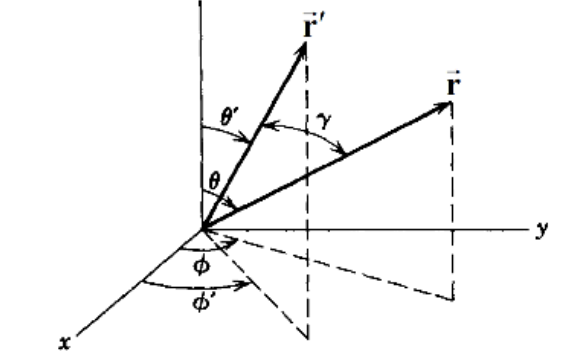
\includegraphics[scale=0.45]{Imagenes/Potencial_Coulomb.png}
    \caption{Sistema de coordenadas empleado en la expansión del potencial de Coulomb.}
    \label{fig:figura_01}
\end{figure}
\end{frame}
\begin{frame}
\frametitle{Manejando el potencial}
Trabajaremos la ec. (\ref{eq:ecuacion_01}) con la finalidad de facilitar la integración:
\begin{eqnarray}
\begin{aligned}[b]
\Phi (\va{r}) &= \scaleint{6ex} \dfrac{\rho(\va{r})}{\abs{\va{r}^{\, \prime} - \va{r}}} \dd{V^{\prime}} = \\[0.5em] \pause
&= \scaleint{6ex} \dfrac{\rho(\va{r})}{\sqrt{r^{\, \prime 2} + r^{2} - 2 r^{\prime} \cdot r}} \dd{V^{\prime}} = \\[0.5em] \pause
&= \scaleint{6ex} \dfrac{\rho(\va{r})}{\sqrt{r^{\, \prime 2} + r^{2} - 2 r^{\prime} \, r \, \cos \gamma }} \dd{V^{\prime}}
\end{aligned}
\label{eq:ecuacion_02}
\end{eqnarray}
\end{frame}
\begin{frame}
\frametitle{Para identificar los valores de $r$}
Indicando con:
\pause
\begin{align*}
r_{<} = \min \left\{ r, r^{\prime} \right\} \hspace{1.5cm} r_{>} = \max \left\{ r, r^{\prime} \right\}
\end{align*}
\end{frame}
\begin{frame}
\frametitle{Expandiendo el denominador}
Expandimos el denominador de la ec. (\ref{eq:ecuacion_02}):
\begin{eqnarray}
\begin{aligned}[b]
\Phi (\va{r}) &= \dfrac{1}{r_{>}} \, \scaleint{10ex} \dfrac{\rho (\va{r}^{\, \prime})}{\sqrt{1 + \bigg( \dfrac{r_{<}}{r_{>}} \bigg)^{2} - 2 \dfrac{r_{<}}{r_{>}} \, \cos \gamma}} \dd{V^{\prime}} = \\[0.5em] \pause
&= \scaleint{6ex} \rho(\va{r}) \, \dfrac{1}{\sqrt{1 + \bigg( \dfrac{r_{<}}{r_{>}} \bigg)^{2} - 2 \dfrac{r_{<}}{r_{>}} \, \cos \gamma}} \dd{V^{\prime}}
\end{aligned}
\label{eq:ecuacion_03}
\end{eqnarray}
\end{frame}
\begin{frame}
\frametitle{Expandiendo el denominador}
Donde:
\pause
\begin{align*}
\cos \gamma = \va{r} \cdot \va{r}^{\, \prime} = \cos \theta \cos \theta^{\prime} +  \sin \theta \sin \theta^{\prime} \cos (\varphi - \varphi^{\prime})
\end{align*}
\end{frame}
\begin{frame}
\frametitle{La función generatriz de los $P_{l}(\cos \theta)$}
Notemos que el denominador de la eq. (\ref{eq:ecuacion_03}) es \emph{la función generadora de los polinomios ordinarios de Legendre}.
\end{frame}
\begin{frame}
\frametitle{La función generatriz de los $P_{l}(\cos \theta)$}
Por lo cual, podemos reescribir el potencial como:
\pause
\begin{eqnarray}
\begin{aligned}[b]
&\Phi (\va{r}) = \dfrac{1}{r_{>}} \, \scaleint{8ex} \rho (\va{r}^{\, \prime}) \, \dfrac{1}{\sqrt{1 + \bigg( \dfrac{r_{<}}{r_{>}} \bigg)^{2} - 2 \dfrac{r_{<}}{r_{>}} \, \cos \gamma}} \dd{V^{\prime}} = \\[0.5em] \pause
&= \dfrac{1}{r_{>}} \nsum_{l=0}^{\infty} \scaleint{8ex} \bigg( \dfrac{r_{<}}{r_{>}} \bigg)^{l} \, \rho (\va{r}^{\, \prime}) \, P_{l} (\cos \gamma) \dd{V}^{\prime}
\end{aligned}
\label{eq:ecuacion_04}
\end{eqnarray}
\end{frame}
\begin{frame}
\frametitle{Integrando la expresión}
Para realizar la integración de la ec. (\ref{eq:ecuacion_04}) reescribimos el $\cos \gamma$, en términos de las variables $\va{r}$ y $\va{r}^{\, \prime}$, para ello usamos el teorema de adición de los armónicos esféricos:
\pause
\begin{align}
P_{l} (\cos \gamma) = \dfrac{4 \pi}{2 \, l + 1} \nsum_{m=-l}^{l} Y_{l}^{m} (\theta^{\prime}, \varphi^{\prime})^{*} \, Y_{l}^{m} (\theta, \varphi)
\label{eq:ecuacion_05}    
\end{align}
\end{frame}
\begin{frame}
\frametitle{Ocupando el teorema de adición}
Entonces al sustituir la ec. (\ref{eq:ecuacion_04}) en la 
ec. (\ref{eq:ecuacion_05}), obtenemos:
\pause
\begin{eqnarray}
\begin{aligned}[b]
\Phi (\va{r}) &=  \nsum_{l=0}^{\infty} \, \nsum_{m=-l}^{l} \dfrac{4 \pi}{2 l {+} 1} \, Y_{l}^{m} (\theta, \varphi) \, \times \\[0.5em]
&\times \scaleint{7ex} \dfrac{(r_{<})^{l}}{(r_{>})^{l+1}} \, \rho (\va{r}^{\, \prime}) \, Y_{l}^{m} (\theta^{\prime}, \varphi^{\prime})^{*} \, r^{\prime 2} \times \\[0.5em]
&\times \sin \theta^{\prime} \dd{r}^{\prime} \dd{\theta}^{\prime} \dd{\varphi}^{\prime}
\end{aligned}
\label{eq:ecuacion_06}
\end{eqnarray}
\end{frame}
\begin{frame}
\frametitle{Resolviendo la integral}
La integración de la ec. (\ref{eq:ecuacion_06} se realiza por casos, tomando en cada uno la correspondiente variable primada en $r_{<}$ y $r_{>}$, \pause la ec.(\ref{eq:ecuacion_06}) es válida para cualquier distribución de carga.
\end{frame}
\begin{frame}
\frametitle{Resolviendo la integral}
Sin embargo estos desarrollos tienen su mayor beneficio en sistemas donde el punto fuente está lejos del punto campo.
\\
\bigskip
\pause
En este caso la estructura de la configuración de carga es irrelevante y se aprecia como un sistema de cargas puntuales.
\end{frame}
\begin{frame}
\frametitle{Resolviendo la integral}
Este proceso se conoce en la literatura como \emph{desarrollo multipolar}, \pause que es la base del estudio de materiales dieléctricos y una de sus aplicaciones es la construcción de la zona de radiación.
\end{frame}

\section{Desarrollo multipolar}
\frame{\tableofcontents[currentsection, hideothersubsections]}
\subsection{Planteamiento de un ejercicio}

\begin{frame}
\frametitle{Caso para el valor de $r$}
Este caso particular corresponde a $\abs{\va{r}^{\, \prime}} = r_{<}$, de tal manera que la ec. (\ref{eq:ecuacion_06}) se reescribe como:
\end{frame}
\begin{frame}
\frametitle{Caso para el valor de $r$}
\begin{align*}
\Phi (\va{r}) &=  \nsum_{l=0}^{\infty} \nsum_{m=-l}^{l} \dfrac{4 \pi}{2 l {+} 1} \dfrac{Y_{l}^{m} (\theta, \varphi)}{r^{l+1}} \times \\[0.5em]
&\times \scaleint{8ex} \rho (\va{r}^{\, \prime}) r^{l+2} Y_{l}^{m} (\theta^{\prime}, \varphi^{\prime})^{*} \sin \theta^{\prime} \dd{r}^{\prime} \dd{\theta}^{\prime} \dd{\varphi}^{\prime} = 
\end{align*}
\end{frame}
\begin{frame}
\frametitle{Caso para el valor de $r$}
\begin{align*}
\Phi (\va{r}) &=  \nsum_{l=0}^{\infty} \nsum_{m=-l}^{l} \dfrac{4 \pi}{2 l {+} 1} \dfrac{Y_{l}^{m} (\theta, \varphi)}{r^{l+1}} \times \\[0.5em]
&\times \bigg[ 
\scaleint{6ex} \rho (\va{r}^{\, \prime}) r^{l+2} Y_{l}^{m} (\theta^{\prime}, \varphi^{\prime})^{*} \sin \theta^{\prime} \dd{r}^{\prime} \dd{\theta}^{\prime} \dd{\varphi}^{\prime} \bigg] = 
\end{align*}
\end{frame}
\begin{frame}
\frametitle{Caso para el valor de $r$}
\begin{align}
\Phi (\va{r}) &=  \nsum_{l=0}^{\infty} \nsum_{m=-l}^{l} \dfrac{4 \pi}{2 l {+} 1} \, \dfrac{q_{l, m} \, Y_{l}^{m}(\theta, \varphi)}{r^{l+1}}
\label{eq:ecuacion_07}
\end{align}
siendo $q_{l,m}$ los momentos multipolares y están definidos por el término entre corchetes.
\end{frame}
\begin{frame}
\frametitle{Caso particular}
Para ilustrar la ec. (\ref{eq:ecuacion_07}), resolvamos un caso particular para la siguiente distribución de carga:
\begin{figure}[H]
    \centering
    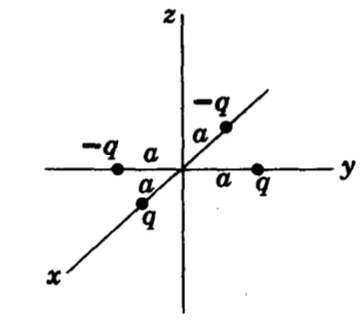
\includegraphics[scale=0.4]{Imagenes/Desarrollo_multipolar_4_cargas.png}
    \caption{Distribución de cargas para el ejercicio.}
    \label{fig:figura_02}
\end{figure}
\end{frame}

\subsection{Resolviendo el problema}

\begin{frame}
\frametitle{Calculando el potencial}
Calculamos el potencial eléctrico de la distribución de carga de la figura (\ref{fig:figura_02}).
\\
\bigskip
\pause
Para este propósito seguimos la ec.(\ref{eq:ecuacion_07}), \pause el primer requisito para el cálculo, \pause es \textcolor{cadetblue}{conocer la densidad de carga}. \pause Recordando que la distribución de carga de una carga puntual es $\rho (\va{r}) = q \, \delta (\va{r})$.
\end{frame}
\begin{frame}
\frametitle{La densidad de carga}
En el caso de la figura (\ref{fig:figura_02}) se tiene que:
\pause    
\begin{eqnarray}
\begin{aligned}[b]
\rho(\va{r}) &= q \, \big[ \delta (x - a) \delta(y) \delta(z) -  \delta (x + a) \delta(y) \delta(z) + \\[0.5em]
&+ \delta (x) \delta(y - a) \delta(z) - \delta (x) \delta(y + a) \delta(z) \big]
\end{aligned}
\end{eqnarray}
\label{eq:ecuacion_08}
\end{frame}
\begin{frame}
\frametitle{Cambiando las deltas de Dirac a esféricas}
Usando la transformación de la delta de Dirac a coordenadas esféricas, la ec. (\ref{eq:ecuacion_08}) la escribimos como:
\end{frame}
\begin{frame}
\frametitle{Cambiando las deltas de Dirac a esféricas}
\begin{align*}
&\rho(\va{r}) = \dfrac{q}{r^{2}} \times \\[0.2em]
&\times \bigg[ \delta(r {-} a) \delta(\cos \theta) \delta(\varphi) {-}  \delta(r {-} a) \delta(\cos \theta) \delta(\varphi {-} \pi) + \\[0.2em]
&+ \delta(r {-} a) \delta(\cos \theta) \delta \bigg(\varphi {-} \dfrac{\pi}{2} \bigg) {-} \\[0.2em]
&+ \delta(r {-} a) \delta(\cos \theta) \delta \bigg( \varphi {-} \dfrac{3 \pi}{2} \bigg) \bigg] = \\[0.2em]
\end{align*}
\end{frame}
\begin{frame}
\frametitle{Cambiando las deltas de Dirac a esféricas}
\begin{align}
\begin{aligned}[b]
&\rho(\va{r}) = \dfrac{q}{r^{2}} \delta(r {-} a) \delta(\cos \theta) \bigg[ \delta \big(\varphi \big) {-} \delta \big(\varphi {-} \pi \big) {+} \\[0.5em]
&+ \delta \bigg( \varphi {-} \dfrac{\pi}{2} \bigg) {-} \delta \bigg(\varphi {-} \dfrac{3 \pi}{2} \bigg) \bigg]
\end{aligned}
\label{eq:ecuacion_09}
\end{align}
\end{frame}
\begin{frame}
\frametitle{Obteniendo los momentos multipolares}
Sustituyendo la ec. (\ref{eq:ecuacion_09}) en la ec. (\ref{eq:ecuacion_07}), obtenemos el cálculo de los momentos multipolares:
\pause
\begin{align*}
&q_{l,m} = \scaleint{5ex} \rho (\va{r}) \, r^{l+2} \, Y_{l}^{m} (\theta, \varphi)^{*} \, \sin \theta \dd{r} \dd{\theta} \dd{\varphi} = 
\end{align*}
\end{frame}
\begin{frame}
\frametitle{Obteniendo los momentos multipolares}
\begin{eqnarray*}
\begin{aligned}
&q_{l,m} = \scaleint{5ex}_{\bs 0}^{2 \pi} \scaleint{5ex}_{\bs 0}^{\pi} \scaleint{5ex}_{\bs 0}^{\infty} q \, \delta(r {-} a) \delta(\cos \theta) \times \\[0.5em] 
&\times \bigg[ \delta \big(\varphi \big) {-} \delta \big(\varphi {-} \pi \big) {+} \delta \bigg( \varphi {-} \dfrac{\pi}{2} \bigg) {-} \delta \bigg(\varphi {-} \dfrac{3 \pi}{2} \bigg) \bigg] \times \\[0.5em]
&\times r^{l} \, Y_{l}^{m} (\theta, \varphi)^{*} \sin \theta \dd{r} \dd{\theta} \dd{\varphi} = \\[0.5em]
\end{aligned}
\end{eqnarray*}
\end{frame}
\begin{frame}
\frametitle{Obteniendo los momentos multipolares}
\begin{eqnarray}
\begin{aligned}[b]
&q_{l,m} = q \, a^{l} \scaleint{5ex}_{\bs 0}^{2 \pi} \scaleint{5ex}_{\bs 0}^{\pi} \delta(\cos \theta) \times \\[0.5em]
&\times \bigg[ \delta \big(\varphi \big) {-} \delta \big(\varphi {-} \pi \big) {+} \delta \bigg( \varphi {-} \dfrac{\pi}{2} \bigg) {-} \delta \bigg(\varphi {-} \dfrac{3 \pi}{2} \bigg) \bigg] \times \\[0.5em]
&\times \, \textcolor{blue}{Y_{l}^{m} (\theta, \varphi)^{*}} \sin \theta \dd{\theta} \dd{\varphi}
\end{aligned}
\label{eq:ecuacion_10}
\end{eqnarray}
\end{frame}
\begin{frame}
\frametitle{Forma explícita del armónico esférico}
Para realizar la integración de la ec. (\ref{eq:ecuacion_10}), debemos de escribir la forma explícita del armónico esférico $\textcolor{blue}{Y_{l}^{m} (\theta, \varphi)^{*}}$:
\pause
\begin{eqnarray*}
\begin{aligned}
&\textcolor{blue}{Y_{l}^{m} (\theta, \varphi)^{*}} = (-1)^{m} \, Y_{l}^{-m} (\theta, \varphi) = \\[0.5em] \pause
&= (-1)^{m} \, \sqrt{\dfrac{2 l + 1}{4 \pi} \, \dfrac{(l + m)!}{(l - m)!}} \, \textcolor{red}{P_{l}^{-m} (cos \theta)} \, e^{-i m \varphi} = 
\end{aligned}
\end{eqnarray*}
\end{frame}
\begin{frame}
\frametitle{Forma explícita del armónico esférico}
\begin{eqnarray}
\begin{aligned}[b]
&\textcolor{blue}{Y_{l}^{m} (\theta, \varphi)^{*}} = (-1)^{m} \, \sqrt{\dfrac{2 l + 1}{4 \pi} \, \dfrac{(l + m)!}{(l - m)!}} \times \\[0.5em]
&\times \textcolor{red}{\bigg[ (-1)^{m} \dfrac{(l - m)!}{(l + m)!} P_{l}^{m} (\cos \theta) \bigg]} \, e^{-i m \varphi} = \\[0.5em] \pause
&= \sqrt{\dfrac{2 l + 1}{4 \pi} \, \dfrac{(l - m)!}{(l + m)!}} \, P_{l}^{m} (\cos \theta) \, e^{-i m \varphi} 
\end{aligned}
\label{eq:ecuacion_11}
\end{eqnarray}
\end{frame}
\begin{frame}
\frametitle{Expresión para el momento multipolar}
Sustituyendo la ec. (\ref{eq:ecuacion_11}) en la ec. (\ref{eq:ecuacion_10}), tendremos que:
\pause
\begin{align*}
&q_{l, m} = q \, a^{l} \scaleint{5ex}_{\bs 0}^{2 \pi} \scaleint{5ex}_{\bs 0}^{\pi} \delta(\cos \theta) \bigg[ \delta \big(\varphi \big) {-} \delta \big(\varphi {-} \pi \big) + \\[0.5em]
&+ \delta \bigg( \varphi {-} \dfrac{\pi}{2} \bigg) {-} \delta \bigg(\varphi {-} \dfrac{3 \pi}{2} \bigg) \bigg] \times \\[0.5em]
&\times \, \textcolor{blue}{Y_{l}^{m} (\theta, \varphi)^{*}} \sin \theta \dd{\theta} \dd{\varphi} = \\[0.5em]
\end{align*}
\end{frame}
\begin{frame}
\frametitle{Expresión para el momento multipolar}
\begin{eqnarray*}
\begin{aligned}
&q_{l, m} = q \, a^{l} \scaleint{5ex}_{\bs 0}^{2 \pi} \scaleint{5ex}_{\bs 0}^{\pi} \delta(\cos \theta) \bigg[ \delta \big(\varphi \big) {-} \delta \big(\varphi {-} \pi \big) + \\[0.5em]
&+ \delta \bigg( \varphi {-} \dfrac{\pi}{2} \bigg) {-} \delta \bigg(\varphi {-} \dfrac{3 \pi}{2} \bigg) \bigg] \times \\[0.5em]
&\times \, \textcolor{red}{\sqrt{\dfrac{2 l + 1}{4 \pi} \, \dfrac{(l - m)!}{(l + m)!}} \, P_{l}^{m} (\cos \theta) \, e^{-i m \varphi}} \sin \theta \dd{\theta} \dd{\varphi} = 
\end{aligned}
\end{eqnarray*}
\end{frame}
\begin{frame}
\frametitle{Expresión para el momento multipolar}
\begin{eqnarray*}
\begin{aligned}
&q_{l, m} = q \, a^{l} \sqrt{\dfrac{2 l + 1}{4 \pi} \, \dfrac{(l - m)!}{(l + m)!}} \, P_{l}^{m} (0) \times \\[0.5em]
&\times \scaleint{6ex} \bigg[ \delta \big(\varphi \big) {-} \delta \big(\varphi {-} \pi \big) {+} \delta \bigg( \varphi {-} \dfrac{\pi}{2} \bigg) - \\[0.5em]
&+ \delta \bigg(\varphi {-} \dfrac{3 \pi}{2} \bigg) \bigg] \, e^{-i m \varphi} \dd{\varphi} = \\[0.5em]
\end{aligned}
\end{eqnarray*}
\end{frame}
\begin{frame}
\frametitle{Expresión para el momento multipolar}
\begin{eqnarray*}
\begin{aligned}
&q_{l,m} = q \, a^{l} \sqrt{\dfrac{2 l + 1}{4 \pi} \, \dfrac{(l - m)!}{(l + m)!}} \, P_{l}^{m} (0) \times \\[0.5em]
&\times \bigg[ 1 - e^{- i \pi m } + \exp \big(- i  \frac{\pi}{2} m \big) - \exp \big(- i \frac{3 \pi}{2} m \big) \bigg] = \\[0.5em] 
\end{aligned}
\end{eqnarray*}
\end{frame}
\begin{frame}
\frametitle{Expresión para el momento multipolar}
\begin{eqnarray*}
\begin{aligned}
&q_{l,m} = q \, a^{l} \sqrt{\dfrac{2 l + 1}{4 \pi} \, \dfrac{(l - m)!}{(l + m)!}} \, P_{l}^{m} (0) \times \\[0.5em]
&\times \big[ 1 {-} i^{m} {-} (-1)^{m} {+} (-1)^{m} \, i^{m}  \big] = \\[0.5em] \pause
&= q \, a^{l} \sqrt{\dfrac{2 l + 1}{4 \pi} \, \dfrac{(l - m)!}{(l + m)!}} \, P_{l}^{m} (0) \big[ 1 - (-1)^{m} \big] \, \big[ 1 - i^{m} \big] = \\[0.5em] \pause
&= 2 \, q \, a^{l} \sqrt{\dfrac{2 l + 1}{4 \pi} \, \dfrac{(l - m)!}{(l + m)!}}\, P_{l}^{m} (0) \big[ 1 - i^{m} \big]
\end{aligned}
\end{eqnarray*}
\end{frame}
\begin{frame}
\frametitle{Ocupando los resultados para el potencial}
Por lo que el potencial se reescribe como:
\pause
\begin{eqnarray}
\begin{aligned}[b]
&\Phi(\va{r}) = \nsum_{l=0}^{\infty} \nsum_{m=-l}^{l} \dfrac{4 \pi}{2 l {+} 1} \times \\[0.5em]
&\times \bigg[ q \, a^{l} \sqrt{\dfrac{2 l + 1}{4 \pi} \, \dfrac{(l - m)!}{(l + m)!}} \times \\[0.5em]
&\times P_{l}^{m} (0) \big[ 1 - i^{m} \big] \bigg] \, \dfrac{Y_{l}^{m} (\theta, \varphi)}{r^{l+1}}
\end{aligned}
\label{eq:ecuacion_12}
\end{eqnarray}
\end{frame}
\begin{frame}
\frametitle{Resolviendo el ejercicio}
Que es lo que se pedía en el ejercicio.
\\
\bigskip
\pause
Observa que para un observador en el eje $z$, \emph{el potencial es nulo}, \pause que es lo que convencionalmente se muestra en los libros elementales de electromagnetismo.
\end{frame}

\subsection{Calculando los momentos multipolares}

\begin{frame}
\frametitle{Momentos multipolares}
Si queremos calcular los momentos multipolares de un arreglo como el de la figura (\ref{fig:figura_02}), tendremos que:
\pause
\begin{align*}
q_{l,m} = q \, a^{l} \sqrt{\dfrac{2 l + 1}{4 \pi} \, \dfrac{(l - m)!}{(l + m)!}} P_{l}^{m} (0) \big[ 1 - i^{m} \big]
\end{align*}
si $m$ es impar, \pause $q_{l,m} = 0$ si $m$ es par.
\end{frame}
\begin{frame}
\frametitle{Momento monopolar}
El momento debido a una carga es:
\pause
\begin{align*}
q_{00} = 0
\end{align*}
ya que $m$ es par.
\\
\bigskip
\pause
Esto tiene sentido, ya que la carga total es cero.
\end{frame}
\begin{frame}
\frametitle{Momentos dipolares}
Los momentos dipolares son:
\pause
\begin{eqnarray*}
\begin{aligned}
q_{1,-1} &= q \, a \, \sqrt{\dfrac{3}{2 \pi}} (1 + i) \\[0.5em] \pause
q_{1,0} &= 0 \\[0.5em] \pause
q_{1,-1} &= q \, a \, \sqrt{\dfrac{3}{2 \pi}} (-1 + i)
\end{aligned}
\end{eqnarray*}
\end{frame}

\end{document}